\chapter{图的分解 (Decompositions of graphs)}

\section{为什么使用图？ (Why graphs?)}

大量现实世界的问题都可以用图（Graph）这种简明而富有表现力的直观语言清晰而精确地描述。例如，考虑对一张政治地图进行着色的问题：在相邻国家必须涂上不同颜色的显而易见限制下，最少需要多少种颜色？解决这一问题的困难之一在于地图本身（哪怕是如图 3.1(a) 所示的简化版地图）通常充斥着大量无关信息：复杂的边界线条、三国或多国交界处的界桩、开阔的海洋以及蜿蜒的河流。而在图 3.1(b) 这一纯粹的数学对象中，这些干扰因素荡然无存——图中的每个顶点对应一个国家（1 代表巴西，11 代表阿根廷），相邻国家之间有一条边连接。它精确地包含了着色所需的全部信息，除此之外别无冗余。此时的精确目标就是为每个顶点分配一种颜色，使得任何一条边的两个端点颜色均不相同。

\begin{figure}[htbp]
\centering
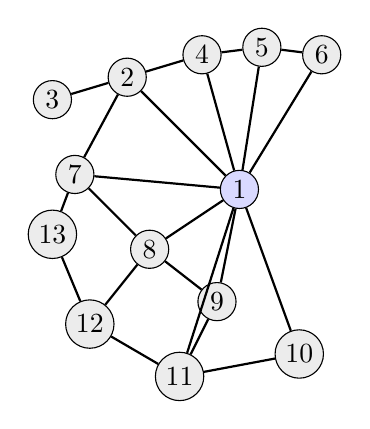
\begin{tikzpicture}[scale=0.95, auto, >=latex]
    % (b) 图模型
    \node[circle,draw,fill=blue!15,inner sep=2pt] (1) at (0,0) {1};
    \node[circle,draw,fill=gray!15,inner sep=2pt] (2) at (-1.5,1.5) {2};
    \node[circle,draw,fill=gray!15,inner sep=2pt] (3) at (-2.5,1.2) {3};
    \node[circle,draw,fill=gray!15,inner sep=2pt] (4) at (-0.5,1.8) {4};
    \node[circle,draw,fill=gray!15,inner sep=2pt] (5) at (0.3,1.9) {5};
    \node[circle,draw,fill=gray!15,inner sep=2pt] (6) at (1.1,1.8) {6};
    \node[circle,draw,fill=gray!15,inner sep=2pt] (7) at (-2.2,0.2) {7};
    \node[circle,draw,fill=gray!15,inner sep=2pt] (8) at (-1.2,-0.8) {8};
    \node[circle,draw,fill=gray!15,inner sep=2pt] (9) at (-0.3,-1.5) {9};
    \node[circle,draw,fill=gray!15,inner sep=2pt] (10) at (0.8,-2.2) {10};
    \node[circle,draw,fill=gray!15,inner sep=2pt] (11) at (-0.8,-2.5) {11};
    \node[circle,draw,fill=gray!15,inner sep=2pt] (12) at (-2.0,-1.8) {12};
    \node[circle,draw,fill=gray!15,inner sep=2pt] (13) at (-2.5,-0.6) {13};

    \draw[thick] (1) -- (2); \draw[thick] (1) -- (4); \draw[thick] (1) -- (5);
    \draw[thick] (1) -- (6); \draw[thick] (1) -- (7); \draw[thick] (1) -- (8);
    \draw[thick] (1) -- (9); \draw[thick] (1) -- (10); \draw[thick] (1) -- (11);
    \draw[thick] (2) -- (3); \draw[thick] (2) -- (4); \draw[thick] (2) -- (7);
    \draw[thick] (4) -- (5); \draw[thick] (5) -- (6); \draw[thick] (7) -- (13);
    \draw[thick] (7) -- (8); \draw[thick] (8) -- (12); \draw[thick] (8) -- (9);
    \draw[thick] (9) -- (11); \draw[thick] (10) -- (11); \draw[thick] (11) -- (12);
    \draw[thick] (12) -- (13);
\end{tikzpicture}
\caption{(a) 地图与其 (b) 抽象图模型}
\label{fig:map_graph}
\end{figure}

图着色绝非地图绘制师的专利。假设一所大学需要为所有课程安排期末考试，并希望使用尽量少的时间段（考场轮次）。唯一的约束条件是：如果某位学生同时选修了两门课程，那么这两门考试就不能安排在同一时间段进行。为了将该问题表示为图，我们为每门考试设立一个顶点，如果存在冲突（即有学生同时选修了这两门课），就在这两个顶点之间连一条边。将每个时间段视为一种独特的颜色。于是，安排考表问题就完全等价于对该图进行顶点着色！

图上的一些基本操作出现的频率极高且应用场景极其广泛，以至于计算机科学家投入了大量精力来寻找它们的高效算法。本章将专门探讨这些算法中最核心的基础算法——那些揭示图的基本连通性结构的算法。

形式上，一个图由顶点集（也称节点集）$V$ 以及连接选定顶点对的边集 $E$ 所定义，记作 $G = (V, E)$。在地图例子中，$V = \{1, 2, 3, \dots, 13\}$，而 $E$ 包含 $\{1, 2\}$、$\{9, 11\}$ 和 $\{7, 13\}$ 等边。这里的边 $\{x, y\}$ 特指“$x$ 与 $y$ 具有共同边界”。这是一种对称关系——它同时也意味着 $y$ 与 $x$ 相邻——我们使用集合记号 $e = \{x, y\}$ 表示。此类边是无向的，包含它们的图称为\textbf{无向图 (undirected graph)}。

有时图所刻画的关系并不具备这种互惠对称性，此时就必须使用带有方向的边。从 $x$ 到 $y$ 的有向边记作 $e = (x, y)$，从 $y$ 到 $x$ 的有向边记作 $(y, x)$。有向图的一个极其宏大的现实范例是万维网（World Wide Web）中所有超链接构成的图：它为互联网上的每个网页设立一个顶点，每当网页 $u$ 包含指向网页 $v$ 的超链接时就存在一条有向边 $(u, v)$——节点和边的总数高达数十亿！理解万维网哪怕最基本的连通性特征，都具有重大的经济与社会价值。虽然该问题的规模庞大得令人望而生畏，但令人欣喜的是，我们将很快看到，许多关于图结构的有价值信息都可以在仅仅\textbf{线性时间}内被求出。

\subsection{图是如何表示的？ (How is a graph represented?)}

我们可以使用\textbf{邻接矩阵 (adjacency matrix)} 来表示图：若图包含 $n = |V|$ 个顶点 $v_1, \dots, v_n$，则邻接矩阵是一个 $n \times n$ 的二维数组 $A$，其第 $(i, j)$ 项定义为：
\[
a_{ij} = \begin{cases}
1, & \text{若存在从 } v_i \text{ 到 } v_j \text{ 的边} \\
0, & \text{否则}.
\end{cases}
\]
对于无向图，邻接矩阵是对称矩阵，因为边 $\{u, v\}$ 可以沿任意方向通行。

\begin{sidebarbox}{你的图有多大？ (How big is your graph?)}
邻接矩阵与邻接表这两种表示法哪一个更好？这取决于图的顶点数 $|V|$ 与边数 $|E|$ 之间的关系。$|E|$ 的取值可以小至 $|V|$（若再小，图就会退化，例如出现孤立点），也可以大至 $\binom{|V|}{2} \approx \frac{|V|^2}{2}$（当所有可能的边都存在时）。当 $|E|$ 接近该范围的上限时，我们称该图为\textbf{稠密图 (dense)}；反之，若 $|E|$ 接近 $|V|$，则称图为\textbf{稀疏图 (sparse)}。正如我们在本章及后续两章中所看到的，图在稠密与稀疏光谱上的确切位置，通常是选择合适图算法的关键决定因素。

对于图的存储表示亦是如此。如果我们要将万维网图存储在计算机内存中，使用邻接矩阵前必须三思：在撰写本书时，搜索引擎已知的万维网顶点约有 80 亿个，因此其邻接矩阵将占据数千万太比特（terabits）。在目前看来，全世界所有计算机内存加起来也难以承受。（寄希望于几年后内存足够大也是不现实的，因为万维网自身会以更快的速度扩张。）

采用邻接表后，存储万维网就变得完全可行了：万维网中总共只有数百亿个超链接，每个超链接在邻接表中仅占几个字节。你可以用一个仅有 1--2 TB 的便携设备装下整个 Web 图结构。邻接表之所以在万维网上极其高效，正是因为\textbf{Web 是高度稀疏的}：在数十亿种可能性中，平均每个网页仅包含指向约半打其他网页的链接。
\end{sidebarbox}

邻接矩阵的最大便利之处在于：检查某条特定边是否存在可以在常数时间 $O(1)$ 内完成（只需一次内存访问）。然而，邻接矩阵需要占据 $O(|V|^2)$ 的空间，如果图的边数很少，这会造成极大的内存浪费。

另一种大小与边数成正比的表示法是\textbf{邻接表 (adjacency list)}。它由 $|V|$ 个链表组成，每个顶点对应一个链表。顶点 $u$ 的链表存放所有由 $u$ 引出的有向边所指向的顶点集合——即满足 $(u, v) \in E$ 的顶点 $v$。因此，若图是有向的，每条边恰好出现在一个链表中；若图是无向的，每条边恰好出现在两个链表中。无论哪种情况，该数据结构的总空间占用均为 $O(|V| + |E|)$。检查某条特定边 $(u, v)$ 是否存在不再是常数时间，因为它需要遍历 $u$ 的邻接链表。但是，遍历一个顶点的所有邻居变得极其容易（只需顺着相应的链表遍历一次即可），我们将很快看到，这在图算法中是一项极其核心且高频的操作。同样，对于无向图，该表示具有对称性：$v$ 在 $u$ 的邻接表中当且仅当 $u$ 在 $v$ 的邻接表中。

\section{无向图的深度优先搜索 (Depth-first search in undirected graphs)}

\subsection{探索迷宫 (Exploring mazes)}
深度优先搜索（DFS）是一种出奇多才多艺的线性时间过程，它能揭示关于图的大量丰富结构信息。它所解决的最基本问题是：
\begin{center}
    \textbf{从给定的起始顶点出发，图的哪些部分是可达的？}
\end{center}
为了理解这一任务，请设想自己是一台刚刚接收到一个新图（比如以邻接表形式给出）的计算机。该表示法仅提供一项基本操作：查找某个顶点的邻居。仅借助这一项原语，可达性问题就像是在探索一座错综复杂的迷宫（图 3.2）。你从一个固定地点出发漫步，每当你到达一个岔路口（顶点）时，都有多条通道（边）可供选择。如果不加小心地选择通道，可能会让你陷入无限打转的死循环，或者遗漏迷宫中某些可达的区域。显然，在探索过程中你需要记录一些中间状态信息。

\begin{figure}[htbp]
\centering
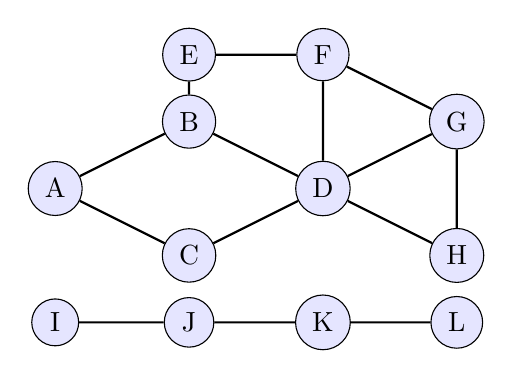
\begin{tikzpicture}[scale=0.85, auto, >=latex]
    \node[circle,draw,fill=blue!10] (A) at (0,2) {A};
    \node[circle,draw,fill=blue!10] (B) at (2,3) {B};
    \node[circle,draw,fill=blue!10] (C) at (2,1) {C};
    \node[circle,draw,fill=blue!10] (D) at (4,2) {D};
    \node[circle,draw,fill=blue!10] (E) at (2,4) {E};
    \node[circle,draw,fill=blue!10] (F) at (4,4) {F};
    \node[circle,draw,fill=blue!10] (G) at (6,3) {G};
    \node[circle,draw,fill=blue!10] (H) at (6,1) {H};
    \node[circle,draw,fill=blue!10] (I) at (0,0) {I};
    \node[circle,draw,fill=blue!10] (J) at (2,0) {J};
    \node[circle,draw,fill=blue!10] (K) at (4,0) {K};
    \node[circle,draw,fill=blue!10] (L) at (6,0) {L};

    \draw[thick] (A)--(B) (A)--(C) (B)--(D) (B)--(E) (C)--(D) (D)--(F) (D)--(G) (D)--(H) (E)--(F) (F)--(G) (G)--(H) (I)--(J) (J)--(K) (K)--(L);
\end{tikzpicture}
\caption{探索图的结构类似于在迷宫中穿行}
\label{fig:maze_graph}
\end{figure}

这一经典挑战在历史上曾吸引了无数人。众所周知，探索迷宫只需要两样法宝：一团线和一盒粉笔。粉笔用于在已访问过的路口做标记，防止绕圈循环；线团则始终指引你返回起点，使你能够回到先前见到但尚未深入调查的岔路通道。

在计算机中我们该如何模拟粉笔和线团这两项原语？粉笔标记很简单：为每个顶点维护一个布尔变量 \texttt{visited}，标识其是否已被访问过。至于线团，在计算机科学中与之完美对应的概念是\textbf{栈 (stack)}。毕竟，线团的确切作用是提供两项操作——放线以深入新路口（在栈中对应于入栈压入新顶点），以及收线以回溯到上一路口（对应于出栈弹出顶点）。

我们无需显式维护一个栈，而是通过\textbf{递归}（利用系统调用栈）隐式地实现它。由此得到的探索算法如图 3.3 所示。\footnote{与我们的许多图算法一样，该算法同时适用于无向图和有向图。在此类通用情形下，我们采用有向边的记号 $(x, y)$。如果图是无向图，则其每条边应被理解为双向同时存在：$(x, y)$ 与 $(y, x)$。} 其中 \texttt{previsit}（前序访问）和 \texttt{postvisit}（后序访问）过程是可选的钩子函数，用于在顶点初次被发现时以及最后彻底离开该顶点时执行特定操作。我们很快会看到它们的精妙用途。

\begin{figure}[htbp]
\centering
\begin{tcolorbox}[colback=white,colframe=gray!50!black,title={\textbf{图 3.3}\quad 探索从特定顶点可达的所有节点 (\texttt{explore})}]
\begin{algorithmic}[1]
\Procedure{explore}{$G, v$}
    \State \textbf{Input:} 图 $G = (V, E)$；起始顶点 $v \in V$
    \State \textbf{Output:} 将所有从 $v$ 可达的节点 $u$ 的 $\text{visited}(u)$ 置为 true
    \State $\text{visited}(v) = \text{true}$
    \State \Call{previsit}{$v$}
    \For{每一条边 $(v, u) \in E$}
        \If{\textbf{not} $\text{visited}(u)$}
            \State \Call{explore}{$u$}
        \EndIf
    \EndFor
    \State \Call{postvisit}{$v$}
\EndProcedure
\end{algorithmic}
\end{tcolorbox}
\label{fig:explore_proc}
\end{figure}

眼下我们需要确认 \texttt{explore} 总是能够正确工作。它显然绝不会走得太远，因为算法仅沿着边从节点走向其邻居，因此绝不可能跳跃到从 $v$ 不可达的区域。但它是否能找出从 $v$ 可达的\textbf{所有}顶点？设想若存在某个它遗漏的可达节点 $u$，在从 $v$ 到 $u$ 的任意路径上，考察该路径上算法实际访问过的最后一个顶点，记作 $z$，并令 $w$ 为该路径上紧随 $z$ 之后的下一个节点：
\[
v \rightsquigarrow z \longrightarrow w \rightsquigarrow u
\]
根据假设，$z$ 被访问了而 $w$ 未被访问。这导致了矛盾：因为当 \texttt{explore} 过程访问节点 $z$ 并扫描其出边时，必定会注意到未被访问的邻居 $w$ 并递归进入它。

顺便提一句，这种推理模式在图论研究中屡见不鲜，本质上是一种流线化的精简归纳法。更形式化的归纳证明会设立归纳假设：“对任意 $k \ge 0$，距离 $v$ 在 $k$ 步跨度以内的所有节点均被访问”。基础情况 $k = 0$ 显然成立（$v$ 自身被访问）；而归纳步（证明若距离为 $k$ 的节点均被访问，则距离为 $k + 1$ 的节点也将被访问）恰好就是我们刚才论证的核心逻辑。

图 3.4 展示了在图 3.2 上从节点 $A$ 开始运行 \texttt{explore} 的结果（当有多个邻居可选时按字母顺序打破平局）。实线边表示实际遍历过的边，每条实线边都由一次 \texttt{explore} 调用触发并导向一个新顶点的发现。例如在访问 $B$ 时，发现了边 $B - E$，由于 $E$ 尚未被访问，算法通过调用 \texttt{explore(E)} 遍历了该边。这些实线边构成了一棵树（无环连通图），因此被称为\textbf{树边 (tree edges)}。虚线边则在探索中被忽略，因为它们指向的是先前已被访问过的熟悉区域，这些边被称为\textbf{回边 (back edges)}。

\begin{figure}[htbp]
\centering
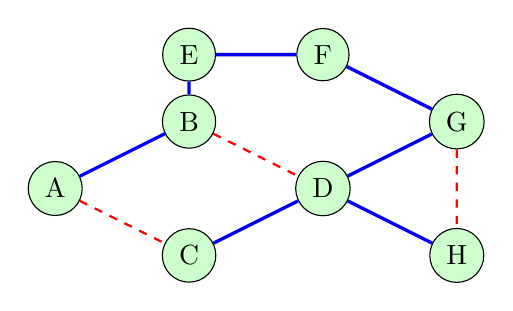
\begin{tikzpicture}[scale=0.85, auto, >=latex]
    \node[circle,draw,fill=green!20] (A) at (0,2) {A};
    \node[circle,draw,fill=green!20] (B) at (2,3) {B};
    \node[circle,draw,fill=green!20] (E) at (2,4) {E};
    \node[circle,draw,fill=green!20] (F) at (4,4) {F};
    \node[circle,draw,fill=green!20] (G) at (6,3) {G};
    \node[circle,draw,fill=green!20] (D) at (4,2) {D};
    \node[circle,draw,fill=green!20] (C) at (2,1) {C};
    \node[circle,draw,fill=green!20] (H) at (6,1) {H};

    % 树边
    \draw[very thick, blue] (A)--(B);
    \draw[very thick, blue] (B)--(E);
    \draw[very thick, blue] (E)--(F);
    \draw[very thick, blue] (F)--(G);
    \draw[very thick, blue] (G)--(D);
    \draw[very thick, blue] (D)--(C);
    \draw[very thick, blue] (D)--(H);

    % 回边
    \draw[thick, dashed, red] (B)--(D);
    \draw[thick, dashed, red] (A)--(C);
    \draw[thick, dashed, red] (G)--(H);
\end{tikzpicture}
\caption{在图 3.2 上执行 \texttt{explore(A)} 得到的 DFS 生成树（蓝色实线为树边，红色虚线为回边）}
\label{fig:dfs_tree_explore}
\end{figure}

\subsection{深度优先搜索 (Depth-first search)}
\texttt{explore} 过程仅仅访问从其起点可达的图部分。为了遍历图的其余部分，我们需要在其他尚未被访问的顶点处重新启动该过程。图 3.5 中称为\textbf{深度优先搜索 (DFS)} 的算法反复执行此操作，直到整张图的所有顶点都被遍历完毕。

\begin{figure}[htbp]
\centering
\begin{tcolorbox}[colback=white,colframe=gray!50!black,title={\textbf{图 3.5}\quad 深度优先搜索 (\texttt{dfs})}]
\begin{algorithmic}[1]
\Procedure{dfs}{$G$}
    \For{所有 $v \in V$}
        \State $\text{visited}(v) = \text{false}$
    \EndFor
    \For{所有 $v \in V$}
        \If{\textbf{not} $\text{visited}(v)$}
            \State \Call{explore}{$G, v$}
        \EndIf
    \EndFor
\EndProcedure
\end{algorithmic}
\end{tcolorbox}
\label{fig:dfs_full}
\end{figure}

分析 DFS 运行时间的第一步是注意到：得益于 \texttt{visited} 数组（粉笔标记），每个顶点恰好被 \texttt{explore} 调用一次。在对某个顶点的探索过程中，包含以下操作：
\begin{enumerate}
    \item 固定常数工作量——标记为已访问，以及执行 \texttt{previsit} / \texttt{postvisit}；
    \item 一个扫描所有相邻边的循环，以检查它们是否通向未访问的新顶点。
\end{enumerate}
该循环对每个顶点耗费的时间各不相同，因此我们将所有顶点统揽合并分析。步骤 1 完成的总工作量为 $O(|V|)$。在步骤 2 中，在整个 DFS 的全过程中，每条无向边 $\{x, y\} \in E$ 恰好被检查两次（一次在 \texttt{explore(x)} 中，一次在 \texttt{explore(y)} 中；若为有向图则每条有向边恰好被检查一次）。因此步骤 2 的总时间为 $O(|E|)$。综合起来，深度优先搜索的运行时间为 $O(|V| + |E|)$，与输入规模呈严格的\textbf{线性关系}。这是我们所能期望的最高效率，因为哪怕仅仅把图的邻接表从头到尾读入一遍也需要这么长时间。

\begin{figure}[htbp]
\centering
\begin{tikzpicture}[scale=0.85, auto, >=latex]
    % (a) 原图
    \begin{scope}[shift={(0,0)}]
        \node[circle,draw,inner sep=2pt] (A) at (0,2) {A}; \node[circle,draw,inner sep=2pt] (B) at (1,2) {B};
        \node[circle,draw,inner sep=2pt] (C) at (2,2) {C}; \node[circle,draw,inner sep=2pt] (D) at (3,2) {D};
        \node[circle,draw,inner sep=2pt] (E) at (0,1) {E}; \node[circle,draw,inner sep=2pt] (F) at (1,1) {F};
        \node[circle,draw,inner sep=2pt] (G) at (2,1) {G}; \node[circle,draw,inner sep=2pt] (H) at (3,1) {H};
        \node[circle,draw,inner sep=2pt] (I) at (0,0) {I}; \node[circle,draw,inner sep=2pt] (J) at (1,0) {J};
        \node[circle,draw,inner sep=2pt] (K) at (2,0) {K}; \node[circle,draw,inner sep=2pt] (L) at (3,0) {L};

        \draw (A)--(B)--(E)--(A) (E)--(I)--(J)--(E) (B)--(J);
        \draw (C)--(D)--(H)--(G)--(C) (D)--(G) (H)--(L)--(K)--(G);
        \node at (1.5, -0.8) {(a) 12 节点图};
    \end{scope}

    % (b) 森林
    \begin{scope}[shift={(6,0)}]
        \node[circle,draw,inner sep=1.5pt,label=above:{\scriptsize 1,10}] (tA) at (0,2) {A};
        \node[circle,draw,inner sep=1.5pt,label=left:{\scriptsize 2,3}] (tB) at (-0.6,1.2) {B};
        \node[circle,draw,inner sep=1.5pt,label=right:{\scriptsize 4,9}] (tE) at (0.6,1.2) {E};
        \node[circle,draw,inner sep=1.5pt,label=left:{\scriptsize 5,8}] (tI) at (0.2,0.4) {I};
        \node[circle,draw,inner sep=1.5pt,label=right:{\scriptsize 6,7}] (tJ) at (0.8,0.4) {J};
        \draw[thick] (tA)--(tB) (tA)--(tE) (tE)--(tI) (tI)--(tJ);

        \node[circle,draw,inner sep=1.5pt,label=above:{\scriptsize 11,22}] (tC) at (2.5,2) {C};
        \node[circle,draw,inner sep=1.5pt,label=right:{\scriptsize 12,21}] (tD) at (2.5,1.2) {D};
        \node[circle,draw,inner sep=1.5pt,label=right:{\scriptsize 13,20}] (tG) at (2.5,0.4) {G};
        \draw[thick] (tC)--(tD)--(tG);

        \node[circle,draw,inner sep=1.5pt,label=above:{\scriptsize 23,24}] (tF) at (4.5,2) {F};
        \node at (2.5, -0.8) {(b) DFS 生成森林};
    \end{scope}
\end{tikzpicture}
\caption{(a) 包含 12 个节点的图及其 (b) DFS 生成森林与前序/后序时间戳}
\label{fig:dfs_forest_undirected}
\end{figure}

图 3.6 展示了在 12 个节点的图上执行 DFS 的结果（同样按字母顺序打破平局）。DFS 的外层循环先后在 $A$、$C$ 以及最后的 $F$ 处调用了三次 \texttt{explore}。结果生成了三棵树，每棵树分别以这三个起始节点为根。它们共同组成了一座\textbf{深度优先生成森林 (forest)}。

\subsection{无向图的连通性 (Connectivity in undirected graphs)}
若无向图中任意两个顶点之间都存在路径，则称该图是\textbf{连通的 (connected)}。图 3.6 中的图显然不是连通的，因为例如从 $A$ 到 $K$ 不存在任何路径。然而，它包含三个互不相交的连通区域，分别对应于以下顶点集合：
\[
\{A, B, E, I, J\}, \quad \{C, D, G, H, K, L\}, \quad \{F\}.
\]
这些区域被称为\textbf{连通分量 (connected components)}：每个连通分量都是一个内部相互连通、但与其余顶点没有任何边相连的极大子图。当从某个特定顶点启动 \texttt{explore} 时，它能精确识别出包含该顶点的整个连通分量。DFS 外层循环每调用一次 \texttt{explore}，就完整提取出一个新的连通分量。

因此，深度优先搜索可以极其简单地改造用于检查图是否连通，并且更一般地，为每个节点 $v$ 赋予一个整数编号 $\text{ccnum}[v]$ 来标识它所属的连通分量。只需定义：
\begin{algorithmic}[1]
\Procedure{previsit}{$v$}
    \State $\text{ccnum}[v] = cc$
\EndProcedure
\end{algorithmic}
其中 $cc$ 在初始时置为 0，并且 DFS 外层循环每次准备调用 \texttt{explore} 时自增 1。

\subsection{前序与后序编号 (Previsit and postvisit orderings)}
我们已经见识了深度优先搜索——区区数行简洁的代码——如何能在短短线性时间内揭示无向图的连通性结构。但它的威力远不止于此。为了进一步挖掘其潜能，我们在探索过程中收集更多信息：对于每个节点，记录下两个重要事件的发生时刻——初次被发现的时刻（对应于 \texttt{previsit}）以及最后彻底离开该节点的时刻（对应于 \texttt{postvisit}）。图 3.6 中标注了这些数字，在包含 12 个节点的图中共有 24 个离散事件。第 5 个事件是发现节点 $I$；第 21 个事件是彻底离开节点 $D$。

利用一个从 1 开始计数的简单全局计数器 \texttt{clock}，可以非常轻松地填充数组 \texttt{pre} 和 \texttt{post}：
\begin{algorithmic}[1]
\Procedure{previsit}{$v$}
    \State $\text{pre}[v] = \text{clock}$
    \State $\text{clock} = \text{clock} + 1$
\EndProcedure
\Procedure{postvisit}{$v$}
    \State $\text{post}[v] = \text{clock}$
    \State $\text{clock} = \text{clock} + 1$
\EndProcedure
\end{algorithmic}

这些时间戳很快会展现出极其重大的意义。与此同时，从图 3.6 中你或许已经注意到了如下基本性质：

\begin{property}
对于任意两个节点 $u$ 和 $v$，两个区间 $[\text{pre}(u), \text{post}(u)]$ 与 $[\text{pre}(v), \text{post}(v)]$ 要么完全不相交，要么其中一个严格包含在另一个之中。
\end{property}
为什么？因为区间 $[\text{pre}(u), \text{post}(u)]$ 本质上就是顶点 $u$ 在递归调用栈中的驻留生命周期。栈的“后进先出”（LIFO）特性自然决定了其区间的嵌套或分离。

\section{有向图的深度优先搜索 (Depth-first search in directed graphs)}

\subsection{边的分类 (Types of edges)}
我们的深度优先搜索算法可以直接原封不动地运行在有向图上，只需注意严格遵循边的指定方向进行遍历。图 3.7 展示了一个有向图示例以及按字母序遍历时生成的搜索树。

\begin{figure}[htbp]
\centering
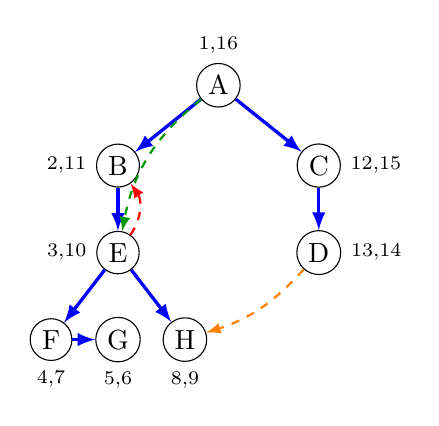
\begin{tikzpicture}[scale=0.85, auto, >=latex]
    % 搜索树节点与时间戳
    \node[circle,draw,inner sep=2pt,label=above:{\scriptsize 1,16}] (A) at (0,3) {A};
    \node[circle,draw,inner sep=2pt,label=left:{\scriptsize 2,11}] (B) at (-1.5,1.8) {B};
    \node[circle,draw,inner sep=2pt,label=right:{\scriptsize 12,15}] (C) at (1.5,1.8) {C};
    \node[circle,draw,inner sep=2pt,label=right:{\scriptsize 13,14}] (D) at (1.5,0.5) {D};
    \node[circle,draw,inner sep=2pt,label=left:{\scriptsize 3,10}] (E) at (-1.5,0.5) {E};
    \node[circle,draw,inner sep=2pt,label=below:{\scriptsize 4,7}] (F) at (-2.5,-0.8) {F};
    \node[circle,draw,inner sep=2pt,label=below:{\scriptsize 5,6}] (G) at (-1.5,-0.8) {G};
    \node[circle,draw,inner sep=2pt,label=below:{\scriptsize 8,9}] (H) at (-0.5,-0.8) {H};

    \draw[->,very thick,blue] (A)--(B); \draw[->,very thick,blue] (B)--(E);
    \draw[->,very thick,blue] (E)--(F); \draw[->,very thick,blue] (F)--(G);
    \draw[->,very thick,blue] (E)--(H); \draw[->,very thick,blue] (A)--(C);
    \draw[->,very thick,blue] (C)--(D);

    % 非树边
    \draw[->,thick,dashed,red] (E) to[bend right=35] (B); % Back edge
    \draw[->,thick,dashed,green!60!black] (A) to[bend right=20] (E); % Forward edge
    \draw[->,thick,dashed,orange] (D) to[bend left=15] (H); % Cross edge
\end{tikzpicture}
\caption{有向图上的 DFS 搜索树及边的分类}
\label{fig:dfs_directed_taxonomy}
\end{figure}

为了进一步分析有向图，引入描述树节点之间关系的术语非常有帮助：$A$ 是搜索树的根（root）；其余所有节点都是它的后代（descendant）。类似地，$E$ 拥有后代 $F, G, H$；反过来，$E$ 是这三个节点的祖先（ancestor）。家庭亲属类比进一步延伸：$C$ 是 $D$ 的双亲（parent），而 $D$ 是其孩子（child）。

在无向图中，我们只区分树边和非树边。而在有向图中，存在更加精细的分类体系（共 4 类边）：
\begin{itemize}
    \item \textbf{树边 (Tree edges)}：实际构成 DFS 生成森林的边；
    \item \textbf{前向边 (Forward edges)}：在 DFS 树中从某个节点指向其非孩子后代节点的边；
    \item \textbf{回边 (Back edges)}：在 DFS 树中从某个节点指向其祖先节点的边；
    \item \textbf{横叉边 (Cross edges)}：既不指向后代也不指向祖先的边；因此它们必定指向一个已经被完全探索完毕（即已经执行过 \texttt{postvisit}）的节点。
\end{itemize}

祖先后代关系以及边的类型可以直接从 \texttt{pre} 和 \texttt{post} 时间戳中读出。由于深度优先探索策略的特性，节点 $u$ 是节点 $v$ 的祖先，恰好对应于 $u$ 先被发现且 $v$ 在 \texttt{explore(u)} 执行期间被发现的情形。也就是说：
\[
\text{pre}(u) < \text{pre}(v) < \text{post}(v) < \text{post}(u),
\]
在几何上表现为嵌套区间 $[ \dots [ \dots ] \dots ]$。下表总结了有向边 $(u, v)$ 的各种时间戳形态与边类型的对应关系：

\begin{center}
\begin{tabular}{cc}
\hline
$(u, v)$ 的前序/后序时间戳区间形态 & 边类型 \\
\hline
$[u \quad [v \quad v] \quad u]$ & 树边 / 前向边 \\
$[v \quad [u \quad u] \quad v]$ & 回边 \\
$[v \quad v] \quad [u \quad u]$ & 横叉边 \\
\hline
\end{tabular}
\end{center}
你想明白为什么不可能出现第 4 种区间形态 $[u \quad u] \quad [v \quad v]$ 了吗？因为如果 $u$ 先结束而 $v$ 后开始，当边 $(u, v)$ 存在时，$u$ 在探索时必定会立刻发现 $v$，而绝不会在未访问 $v$ 的情况下就提前结束离开！

\subsection{有向无环图 (Directed acyclic graphs)}
有向图中的环路（有向环，cycle）是指一条首尾相接的闭合路径 $v_0 \to v_1 \to v_2 \to \dots \to v_k \to v_0$。不包含任何环图的有向图称为\textbf{有向无环图 (Directed Acyclic Graph，简称 DAG)}。事实证明，我们只需一次深度优先搜索，就能在线性时间内判定一个图是否为 DAG。

\begin{property}
一个有向图包含环路，当且仅当对其进行深度优先搜索时出现了回边 (back edge)。
\end{property}

\begin{proof}
充分性（$\Leftarrow$）非常直接：若 $(u, v)$ 是一条回边，则 $v$ 是 $u$ 的祖先，因此搜索树中从 $v$ 到 $u$ 的路径连同该边 $(u, v)$ 立即构成一个有向环。

必要性（$\Rightarrow$）：若图中包含环路 $v_0 \to v_1 \to \dots \to v_k \to v_0$，考察该环上最早被 DFS 发现的节点（即拥有最小 \texttt{pre} 值的节点），设为 $v_i$。环上其余所有节点 $v_j$ 都可以从 $v_i$ 出发沿着环路到达，因此在以 $v_i$ 为根的搜索子树中它们都将成为 $v_i$ 的后代。特别地，环上的前驱边 $v_{i-1} \to v_i$（若 $i = 0$ 则为 $v_k \to v_0$）是从一个后代节点指向其祖先节点 $v_i$ 的边，根据定义，这必定是一条回边。
\end{proof}

有向无环图（DAG）在现实中无处不在。它们非常适合对因果关系、层级结构和时间依赖性进行建模。例如，假设你需要完成多项任务，但某些任务必须在其他任务完成后才能开始（你必须先醒来才能起床；必须起床后才能穿衣洗漱等等）。此时的问题是：是否存在一个合法的任务执行顺序？

这类约束可以非常自然地表示为一个有向图：每个任务对应一个节点，若 $u$ 是 $v$ 的前置先决条件，则连一条边 $u \to v$。也就是说，在执行任务 $v$ 之前，所有指向它的任务都必须已完成。如果这个图包含环路，那就彻底陷入死锁僵局（没有可行的顺序）。反之，如果该图是一个 DAG，我们希望对其进行\textbf{拓扑排序 (Topological sort，或称线性化 Linearization)}——即将顶点排成一条线，使得图中的每一条有向边都严格从靠前的顶点指向靠后的顶点。

\begin{property}
在 DAG 中，每一条有向边 $(u, v)$ 都满足 $\text{post}(u) > \text{post}(v)$。
\end{property}

这为我们提供了一个对 DAG 进行拓扑排序的线性时间算法：\textbf{只需对图运行 DFS，然后按照后序编号（\texttt{post} 值）从大到小的降序排列输出所有顶点即可}。

由于 DAG 是按照 \texttt{post} 值递减线性化的，因此拥有最小 \texttt{post} 值的节点必定排在序列的最末端，它必然是一个\textbf{汇点 (sink)}——没有任何出边。对称地，拥有最大 \texttt{post} 值的节点必然是一个\textbf{源点 (source)}——没有任何入边。

\begin{property}
任何有向无环图 (DAG) 至少包含一个源点 (source) 和至少一个汇点 (sink)。
\end{property}

源点的存在性启发了拓扑排序的另一种等价思路：找到一个源点，输出它，将其从图中删除，然后重复该过程直到图为空。

\section{强连通分量 (Strongly connected components)}

\subsection{有向图连通性的定义}
在无向图中，连通性的定义极为直观：非连通图可以自然地分解为若干个互不相交的连通分量。而在有向图中，连通性要微妙得多。在图 3.9(a) 中，虽然图在直观上不能被“扯断”，但它显然不能被视为连通的，因为例如从 $G$ 到 $B$ 或从 $F$ 到 $A$ 根本不存在任何路径。

有向图连通性的正确定义应当是：
\begin{center}
    \textbf{若有向图中节点 $u$ 到 $v$ 存在路径，且 $v$ 到 $u$ 也存在路径，则称 $u$ 与 $v$ 是强连通的。}
\end{center}

该关系在顶点集 $V$ 上构成了等价关系，它将 $V$ 划分为若干个互不相交的等价类，称为\textbf{强连通分量 (Strongly Connected Components，简称 SCC)}。

\begin{figure}[htbp]
\centering
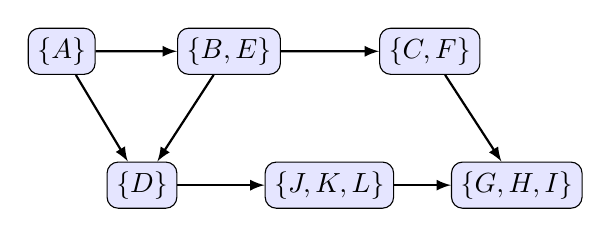
\begin{tikzpicture}[scale=0.85, auto, >=latex]
    % 元图 DAG
    \node[draw,rectangle,rounded corners,fill=blue!10] (S1) at (0,2) {$\{A\}$};
    \node[draw,rectangle,rounded corners,fill=blue!10] (S2) at (2.5,2) {$\{B, E\}$};
    \node[draw,rectangle,rounded corners,fill=blue!10] (S3) at (5.5,2) {$\{C, F\}$};
    \node[draw,rectangle,rounded corners,fill=blue!10] (S4) at (1.2,0) {$\{D\}$};
    \node[draw,rectangle,rounded corners,fill=blue!10] (S5) at (4.0,0) {$\{J, K, L\}$};
    \node[draw,rectangle,rounded corners,fill=blue!10] (S6) at (6.8,0) {$\{G, H, I\}$};

    \draw[->,thick] (S1)--(S2); \draw[->,thick] (S1)--(S4); \draw[->,thick] (S2)--(S3);
    \draw[->,thick] (S2)--(S4); \draw[->,thick] (S3)--(S6); \draw[->,thick] (S4)--(S5);
    \draw[->,thick] (S5)--(S6);
\end{tikzpicture}
\caption{有向图收缩后得到的强连通分量元图 (Meta-graph) 必为 DAG}
\label{fig:meta_dag}
\end{figure}

现在将每个强连通分量收缩为一个“元节点”（meta-node），若分量之间存在有向边，就在对应的元节点之间连边。由此得到的\textbf{元图 (meta-graph) 必定是一个 DAG}！因为如果元图包含环路，那么环上的所有强连通分量就会全部合并为单个更大的强连通分量。

\begin{property}
任何有向图都是其强连通分量构成的有向无环图 (DAG)。
\end{property}

这揭示了一个核心认知：\textbf{有向图的连通结构是两层的}。宏观顶层是一个 DAG（结构清晰，可拓扑排序）；微观底层则是每个元节点内部高度连通的强连通分量。

\subsection{高效的强连通分量算法 (Kosaraju-Sharir 算法)}

\begin{property}
在深度优先搜索中，获得全局最大 \texttt{post} 编号的节点，必定位于元图的某个\textbf{源点强连通分量 (source SCC)} 中。
\end{property}

为了找到强连通分量，如果我们从一个\textbf{汇点强连通分量 (sink SCC)} 中的节点启动 \texttt{explore}，搜索就会被局限在该分量内部，从而恰好完整提取出该分量！但如何找到汇点分量？

答案是利用\textbf{反向图 (Reverse graph)} $G^R$：即保持顶点集不变，将所有边的方向反转。$G^R$ 拥有与 $G$ 完全相同的强连通分量。在 $G^R$ 上的源点强连通分量，恰好就是原图 $G$ 中的汇点强连通分量！

由此诞生了极其优美高效的强连通分量线性时间算法：
\begin{enumerate}
    \item 对反向图 $G^R$ 运行深度优先搜索，记录每个顶点的 \texttt{post} 时间戳；
    \item 按照在步骤 1 中计算出的 \texttt{post} 值从大到小的降序，在原图 $G$ 上依次调用 \texttt{explore} 过程。每次调用所遍历到的未访问节点集合就是一个独立的强连通分量。
\end{enumerate}
该算法的总时间复杂度为 $O(|V| + |E|)$，是严格线性的！

\begin{sidebarbox}{快速网络爬虫 (Crawling fast)}
在真实的万维网搜索引擎爬虫中，图的节点事先未知，必须在爬取过程中动态发现。爬虫维护一个显式队列或优先级队列来管理待抓取的 URL，使用哈希表快速判定某网页是否已访问过，并利用强连通分量算法分析 Web 的宏观拓扑结构。
\end{sidebarbox}

\newpage
\section*{习题 (Exercises)}
\addcontentsline{toc}{section}{习题}

\begin{exercise}{3.1}
对给定无向图执行深度优先搜索（字母序打破平局），将每条边分类为树边或回边，并给出每个顶点的 \texttt{pre} 和 \texttt{post} 编号。
\end{exercise}

\begin{exercise}{3.2}
对两个给定的有向图执行 DFS，将每条边分类为树边、前向边、回边或横叉边，并记录各顶点时间戳。
\end{exercise}

\begin{exercise}{3.3}
对给定 DAG 运行基于 DFS 的拓扑排序算法：(a) 给出节点的 \texttt{pre} 和 \texttt{post} 编号；(b) 指出图中的源点与汇点；(c) 给出算法求得的拓扑排序序列；(d) 该图总共拥有多少种不同的合法拓扑排序？
\end{exercise}

\begin{exercise}{3.4}
在给定的有向图上运行强连通分量算法：(a) 写出 SCC 被发现的顺序；(b) 指出哪些是源 SCC，哪些是汇 SCC；(c) 绘制元图；(d) 最少需要添加多少条边才能使整个图变为强连通图？
\end{exercise}

\begin{exercise}{3.5}
给出在线性时间 $O(|V| + |E|)$ 内计算邻接表格式图的反向图 $G^R$ 的算法。
\end{exercise}

\begin{exercise}{3.6}
握手定理与度数：(a) 证明无向图中 $\sum_{u \in V} d(u) = 2|E|$；(b) 证明奇数度顶点的个数必定为偶数；(c) 有向图的入度是否有类似性质？
\end{exercise}

\begin{exercise}{3.7}
二分图（Bipartite graph）：(a) 给出判断无向图是否为二分图的线性时间算法；(b) 证明图是二分图当且仅当它不包含奇数长度的环；(c) 恰好包含一个奇环的无向图最多需要几种颜色着色？
\end{exercise}

\begin{exercise}{3.8}
倒水问题：三个容量分别为 10、7、4 品脱的容器，初始状态为 $(0, 7, 4)$。将其建模为图搜索问题并求解。
\end{exercise}

\begin{exercise}{3.9}
在邻接表下，设计线性时间算法计算每个节点的“二阶度”（即所有邻居的度数之和）。
\end{exercise}

\begin{exercise}{3.10}
使用显式栈将 \texttt{explore} 过程改写为非递归版本，保持 \texttt{previsit} 与 \texttt{postvisit} 的调用时机和效果完全不变。
\end{exercise}

\begin{exercise}{3.11}
设计线性时间算法，判断无向图中是否存在包含指定边 $e$ 的简单环。
\end{exercise}

\begin{exercise}{3.12}
证明或给出反例：若 $\{u, v\}$ 为无向图的一条边，且在 DFS 中 $\text{post}(u) < \text{post}(v)$，则 $v$ 必为 $u$ 在搜索树中的祖先。
\end{exercise}

\begin{exercise}{3.13}
无向与有向连通性对比：(a) 证明连通无向图必存在一个可删除而不破坏连通性的顶点；(b) 给出强连通有向图的反例；(c) 探讨添加一条边对连通分量的影响。
\end{exercise}

\begin{exercise}{3.14}
展示如何在线性时间内实现通过反复删除源点来进行拓扑排序的算法。
\end{exercise}

\begin{exercise}{3.15}
单行道城市交通网络建模：(a) 判定任意两个路口是否均可互相到达（强连通性判定）；(b) 弱连通性性质判定。
\end{exercise}

\begin{exercise}{3.16}
先修课程图与最短毕业学期数：在 DAG 上设计线性时间算法计算完成所有先修依赖课程所需的最少学期数（最长路径问题）。
\end{exercise}

\begin{exercise}{3.17}
无限路径与模型检测（$\omega$-automata 基础）：分析无限轨迹的极限集合 $\text{Inf}(p)$ 与强连通分量的关系。
\end{exercise}

\begin{exercise}{3.18}
有根树的祖先查询预处理：设计线性时间预处理算法，使得“$u$ 是否为 $v$ 的祖先”查询可在 $O(1)$ 常数时间内完成。
\end{exercise}

\begin{exercise}{3.19}
树上子树极值查询：在线性时间内计算每个节点的所有后代节点的最大权值。
\end{exercise}

\begin{exercise}{3.20}
树上 $k$ 级祖先标签更新问题。
\end{exercise}

\begin{exercise}{3.21}
设计线性时间算法寻找有向图中的奇数长度环。
\end{exercise}

\begin{exercise}{3.22}
设计高效算法判断有向图中是否存在一个能够到达所有其他顶点的“超级源点” $s$。
\end{exercise}

\begin{exercise}{3.23}
给定 DAG 和顶点 $s, t$，设计线性时间算法统计从 $s$ 到 $t$ 的不同有向路径总数。
\end{exercise}

\begin{exercise}{3.24}
判定 DAG 中是否存在一条恰好访问每个顶点一次的有向哈密顿路径。
\end{exercise}

\begin{exercise}{3.25}
有向图上的最小代价可达节点计算（DAG 线性算法推广至一般有向图）。
\end{exercise}

\begin{exercise}{3.26}
欧拉回路与哥尼斯堡七桥问题：证明无向图存在欧拉回路当且仅当所有顶点度数均为偶数。
\end{exercise}

\begin{exercise}{3.27}
证明在无向图中可以将奇数度的顶点两两配对，使得它们之间的路径相互边不相交。
\end{exercise}

\begin{exercise}{3.28}
\textbf{2SAT 问题的强连通分量线性时间解法}：将 2-CNF 规约到蕴含图 $G_I$，证明可满足性充要条件为任何变量 $x$ 与 $\neg x$ 均不属于同一个 SCC。
\end{exercise}

\begin{exercise}{3.29}
等价关系与无向图连通分支划分。
\end{exercise}

\begin{exercise}{3.30}
证明有向图上的相互可达关系是等价关系。
\end{exercise}

\begin{exercise}{3.31}
\textbf{双连通分量、割点与桥}：利用 DFS 时间戳与 $\text{low}(u)$ 数组在线性时间内求出无向图的所有割点（关节点）、桥与双连通分量（Tarjan 算法）。
\end{exercise}
